\documentclass[twocolumn]{article}
%%
%% Language and font encodings
\usepackage{tgtermes} 
\usepackage[english]{babel}
\usepackage[utf8x]{inputenc}
\usepackage[T1]{fontenc}

%% enumerate
\usepackage{enumerate} 
%% figure caption
\usepackage[font=small,labelfont=bf]{caption}

%% Sets page size and margins
\usepackage[a4paper,top=3cm,bottom=2cm,left=3cm,right=3cm,marginparwidth=1.75cm]{geometry}
\usepackage{indentfirst}
\usepackage{listings}
\lstset{ 
	language=Matlab,                		% choose the language of the code
%	basicstyle=10pt,       				% the size of the fonts that are used for the code
	numbers=left,                  			% where to put the line-numbers
	numberstyle=\footnotesize,      		% the size of the fonts that are used for the line-numbers
	stepnumber=1,                   			% the step between two line-numbers. If it's 1 each line will be numbered
	numbersep=5pt,                  		% how far the line-numbers are from the code
%	backgroundcolor=\color{white},  	% choose the background color. You must add \usepackage{color}
	showspaces=false,               		% show spaces adding particular underscores
	showstringspaces=false,         		% underline spaces within strings
	showtabs=false,                 			% show tabs within strings adding particular underscores
%	frame=single,	                			% adds a frame around the code
%	tabsize=2,                				% sets default tabsize to 2 spaces
%	captionpos=b,                   			% sets the caption-position to bottom
	breaklines=true,                			% sets automatic line breaking
	breakatwhitespace=false,        		% sets if automatic breaks should only happen at whitespace
	escapeinside={\%*}{*)}          		% if you want to add a comment within your code
}
\usepackage{pgfplotstable}
\usepackage{indentfirst}
\usepackage{float}
\usepackage{subfigure}
%% Useful packages
\usepackage{amsmath}
\usepackage{graphicx}
\usepackage[colorinlistoftodos]{todonotes}
\usepackage[colorlinks=true, allcolors=blue]{hyperref}

\title{Scheduling Algorithms for Image Precessing }
\author{Zeng Qiuhao \& Chang Shuning}
\date{\today}

\begin{document}

\makeatletter
    \begin{titlepage}
        \begin{center}
        \vspace*{20mm}
            
\includegraphics[width=0.7\linewidth]{walala.jpg}\\[20ex]
            {\huge \bfseries  \@title }\\[5ex] 
            {\LARGE  \@author}\\[4ex] 
            {\LARGE  A0169256U\& A0177243A}\\[4ex] 
            {\LARGE  e0178343@u.nus.edu \& e0251087@u.nus.edu}\\[40ex] 
            {\large \@date}
        \end{center}
    \end{titlepage}
\makeatother
\thispagestyle{empty}
\newpage
\section{Abstract}
% Must capture the aim,
% objective and algorithms
% used and highlight of
% results
Most image processing algorithms are computational drastic and require significant computing power. Parallel architectures can contribute higher processing power. For the first part, following the recently evolved paradigm, referred to as divisible load theory (DLS), we survey the Branch and Bound LifoC Algorithm for parallel image processing on heterogeneous network systems. However, parallel architecture is not always a cost-effective way because of possible high communication time. We also survey an uniprocessor algorithm. 
For the second part, we will discuss about an adaptive scheduling method using anytime algorithm under a condition that the processing time is restricted or is not enough. We will establish a modeling of time precision function, which will realize the maximum performance in the restricted time.By comparison with two algorithms under different situations, we analyze their property.




\section{Introduction}
% 1.Need for the problem,
% motivation, Clear problem
% statement(s) – plain
% English; 2. Problem
% statement using technical
% description (formulation
% of an objective func with
% constraints, etc); Cite the
% papers you used at the
% appropriate places; You
% may open sub-sections as
% you see fit.
\subsection{First Part}
\subsubsection{Divisible Load Theory}
Divisible loads form a special class of parallelizable applications, which if given a large enough volume, can be arbitrarily partitioned into any number of independently and identically processable load fractions. Examples of applications that satisfy this divisibility property include massive dataset processing, image processing. Divisible load theory(DLT) is the mathematical framework that has been established to study divisible load scheduling(DLS).

DLT has gained popularity because of its simplicity and deterministic nature. In a star connected network where the center of the star acts as the master and holds the entire load to be distributed, and the points of the star form the set of slave processors.

Processors can communication with only one other processor at the time, and communication and computation cannot occur simultaneously. If the allocated image fraction is $\alpha_k$, then the returned result is equal to $\delta\alpha_k$, where $0\le\alpha\le 1$. The constant $\delta$ is application specific, and is the same for all processors for a particular image size L. For an image part $\alpha_k, C_k \alpha_k$ is the transmission time from $P_0$ to $P_k, E_k, \alpha_k$ is the time it tales $P_k$ to perform the requisite processing on $\alpha_k$, and $\delta C_k \alpha_k$ is the time it takes $P_k$ to transmit the image results back to $P_0$.
  $\sigma_a$ and $\sigma_c$ are two permutation of order m that represent the allocation and collection sequences respectively $\sigma_a [k]$ and $\sigma_c [k]$ denote the processor number that occurs at index $k\in\{1,⋯,m\}$. $\sigma_a [k]$ and $\sigma_c [k]$ are two lookup functions that return the index of the processor k in the allocation and collection sequences. Purpose of scheduling is to find the sequence pair $(\sigma_a, \sigma_c)$, and $\alpha_([1⋯m])$ that minimize total processing time.


\subsubsection{System Mode}
The network model to be considered here consists of (M+1) processors interconnected through M links in a single-level tree fashion as show in Figure below.

\begin{figure}[H]
\centering
  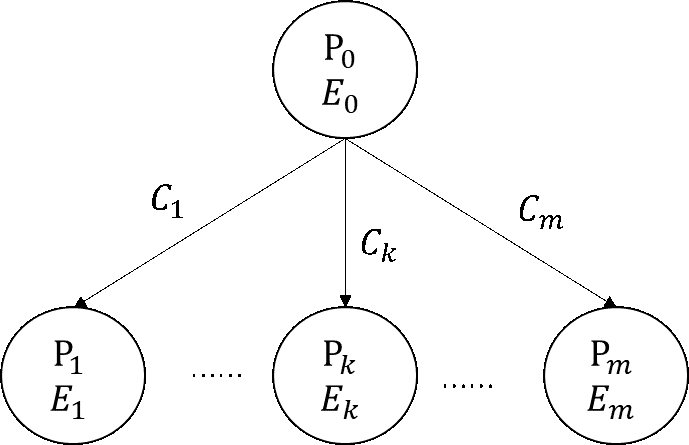
\includegraphics[width=0.4\textwidth]{csn1.png}
\caption{A heterogeneous star network}
\end{figure}

Where $P=\{P_0,⋯,P_m\}$ is the set of m+1 processors, and $E=\{E_0,⋯,E_m\}$ is the set of computation parameters of the slave processors, and $C={C_0,⋯,C_m}$ is the set of communication parameters of the network links. $E_k$ is the reciprocal of the speed of processor $P_k$ and $C_k$ is the reciprocal of the bandwidth of the link. Both are defined in time units per unit load, that is, $P_k$ takes $E_k$ time units to process a unit load transmitted to it from $P_0$ in $C_k$ time units over the same link. It follows that $\forall k \in\{1,...,m\}$: $E_k > 0, C_k > 0$. In this model, L is the whole image size that exists in master computer. Since it does not damage problem, we suppose that L=1. The source $P_0$ splits L into parts and sends them to the respective processors $P_1,⋯,P_m$ for processing. Each such set of m parts known as a load distribution $\alpha=\{\alpha_1,\alpha_2,⋯,\alpha_m\}$.

\subsection{Second Part}
\subsubsection{Goal and Problem Clarification}
For the first part, as the quality of image processing is usually evaluated by high extraction rate or low error rate. We perform individual image processing task at optimal time, in order to be able to output the result at midway processing time.  It also describes an evaluation method under such a condition that the processing time is restricted or is not enough, and proposes an adaptive scheduling method by using anytime algorithmic image processing. The new technique which output the result where performance becomes best within the tact is actualized according to the definition of anytime algorithms. 

\subsubsection{Performance Model}
To establish the performance model, we cite another paper\cite{Using anyt}\relax. A performance profile of an anytime algorithm, Q(t), denotes the expected output quality with execution time t. And Performance Profiles are typically constructed empirically by collecting statistics on the performance of an algorithm over many input instances. 

Here I mainly investigate two operators. The smoothing operator (single averaging) Process using 3 by 3 mask:

\begin{figure}[H]
\centering
  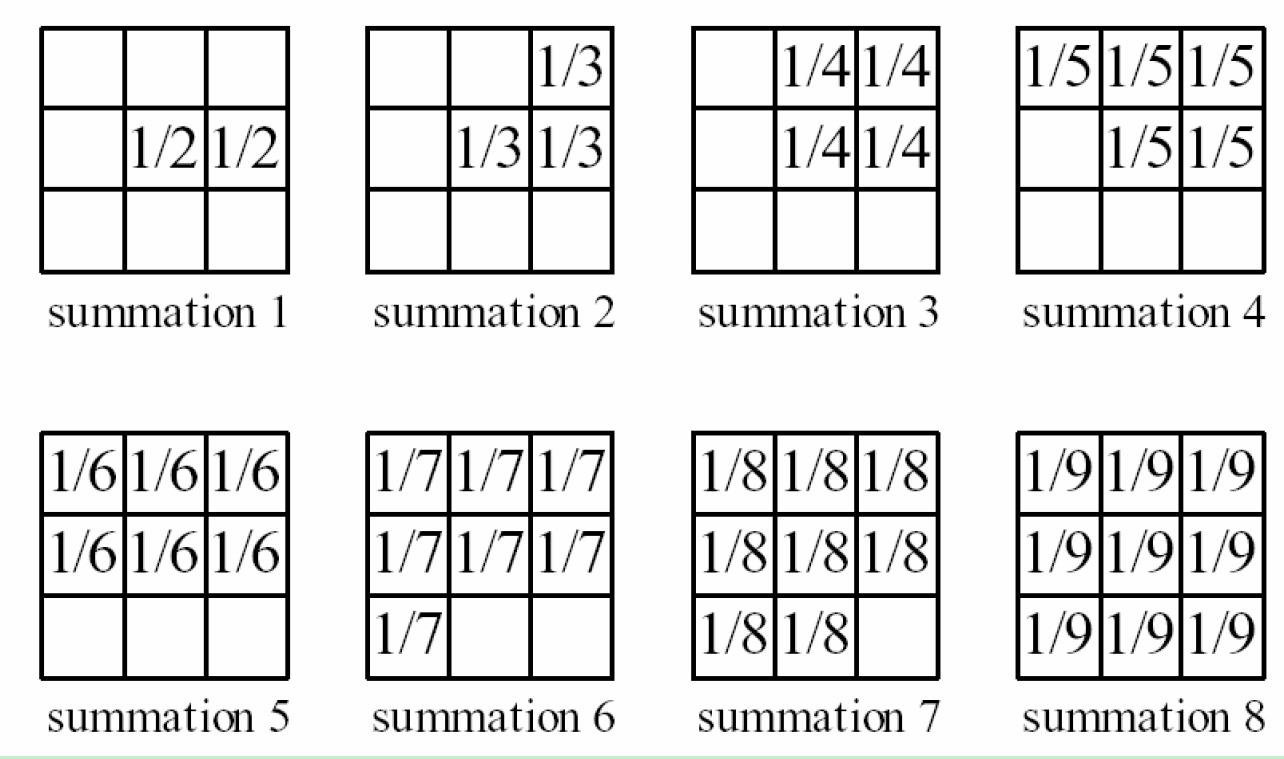
\includegraphics[width=0.4\textwidth]{sum.jpg}
\caption{An Example of A Set of Anytime Algorithmic Smoothing Operator}
\end{figure}

Via simulation, I get the statistics on the performance related to time (worst-case execution time of three results)
\begin{table}[h!]
\centering
\scalebox{0.4}{
\begin{tabular}{ cccccccc } 
 \hline
  Smoothing Operator& Summation 1& Summation 2 & Summation 3& Summation 4& Summation 5& Summation 6& Summation 7\\ 
  \hline
WCET/s & 1 & 1.3 & 1.75 & 2.4&3.1&4.05&5 \\
 Performance &0.2& 0.4  & 0.5 & 0.62 & 0.68 & 0.8 & 1\\ 
 \hline
\end{tabular}
}
\caption{Performance with Different Smoothing Operator}
\end{table}

With MATLAB Fitting Tool, I define Q(t) for smoothing operator for this image as 1 order polynomial:
\begin{equation*}
Q(t) =  0.1733t-0.1394
\end{equation*}

\begin{figure}[H]
\begin{minipage}{0.48\linewidth}
  \centerline{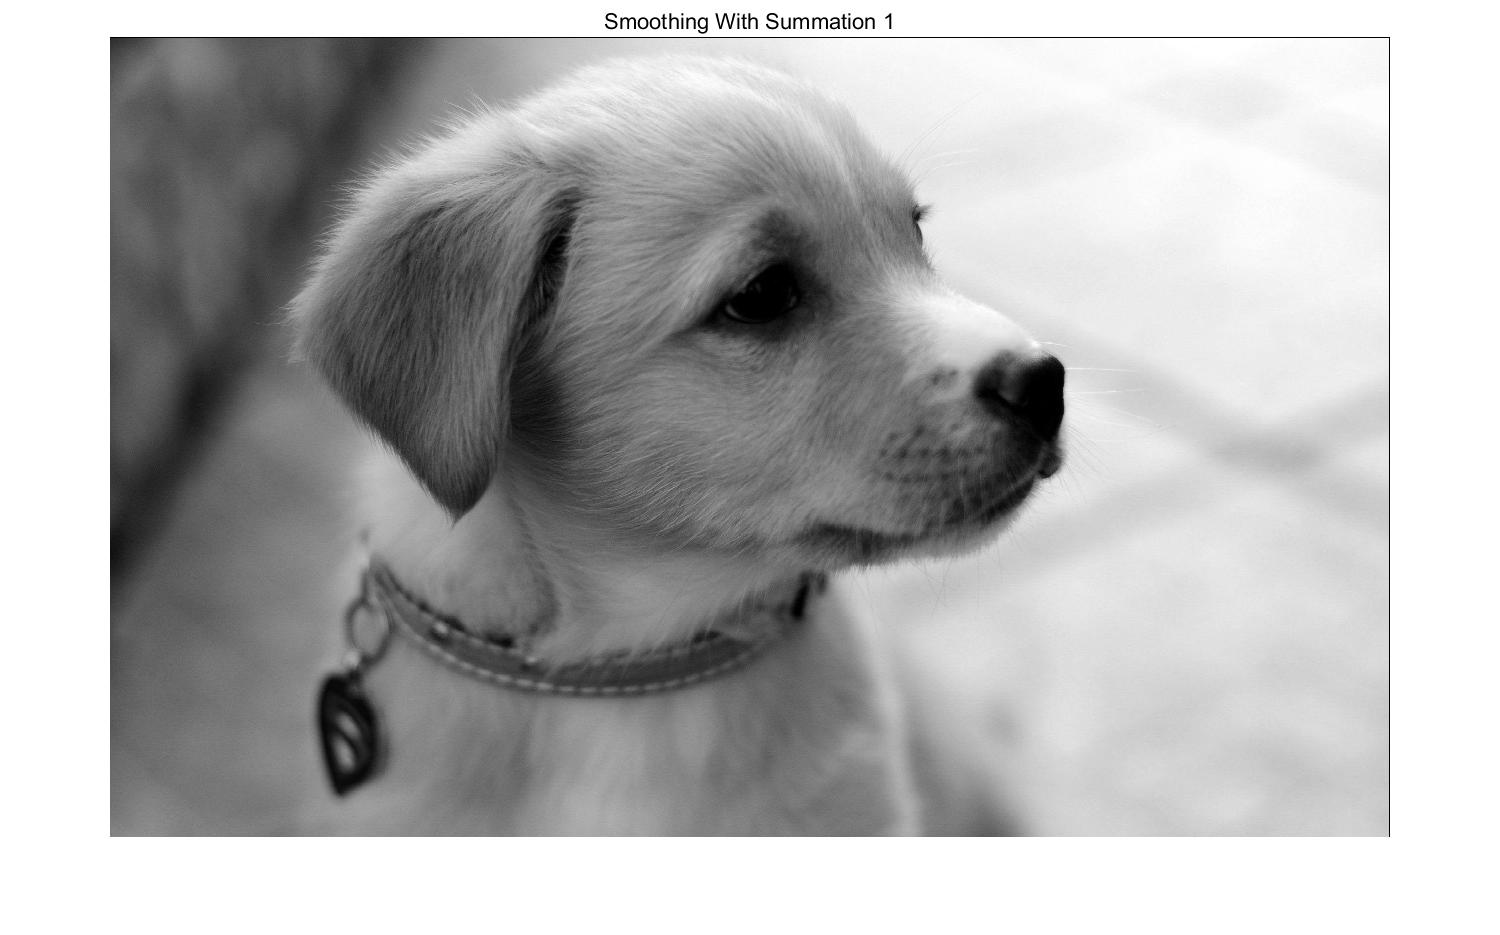
\includegraphics[width=4.0cm]{sum1.jpg}}
  \centerline{(a) Summation 1}
\end{minipage}
\hfill
\begin{minipage}{0.48\linewidth}
  \centerline{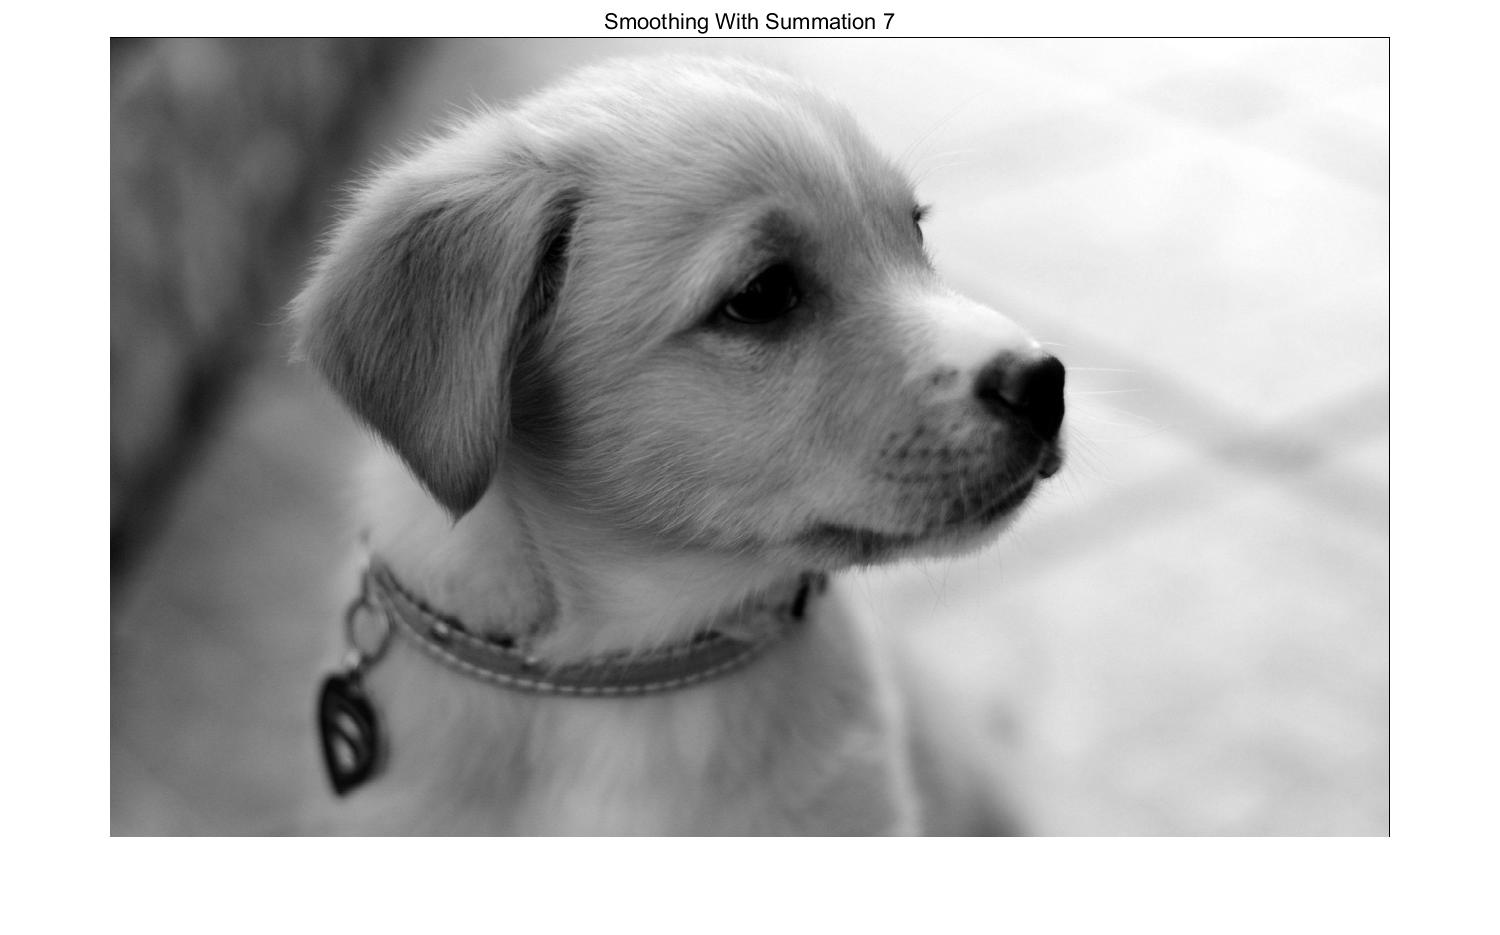
\includegraphics[width=4.0cm]{sum7.jpg}}
  \centerline{(b) Summation 7}
\end{minipage}
 \caption{Results of Summation 1 and 7}
\end{figure}

Also I investigate the edge detection operator:
\begin{equation*}
g = \sqrt{vertical^2+horizontal^2}
\end{equation*}

\begin{figure}[H]
\centering
  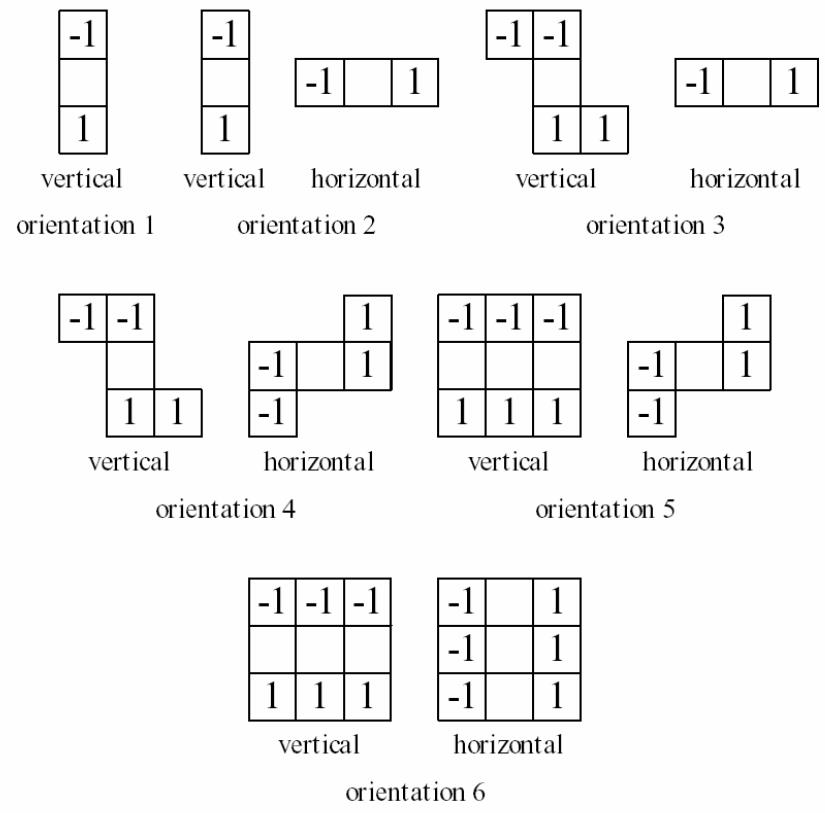
\includegraphics[width=0.4\textwidth]{orientation.jpg}
\caption{An Example of A Set of Anytime Algorithmic Edge Detection Operator}
\end{figure}

\begin{table}[h!]
\centering
\scalebox{0.5}{
\begin{tabular}{ ccccccc} 
 \hline
  Detection Operator& Orientation 1 & Orientation 2 & Orientation 3 & Orientation 4 & Orientation 5 & Orientation 6\\ 
  \hline
WCET &1.5 &1.7&2.1&2.7 &3.6&5 \\
 Performance & 0.11&0.22&0.54& 0.83 & 0.96 & 1 \\ 
 \hline
\end{tabular}
}
\caption{Performance with Different Detection Operator}
\end{table}

With MATLAB Fitting Tool, for simplicity I define Q(t) for edge detection operator for this image as 1 order polynomial:
\begin{equation*}
Q(t) = 0.2529t-0.08967
\end{equation*}

\begin{figure}[H]
\begin{minipage}{0.48\linewidth}
  \centerline{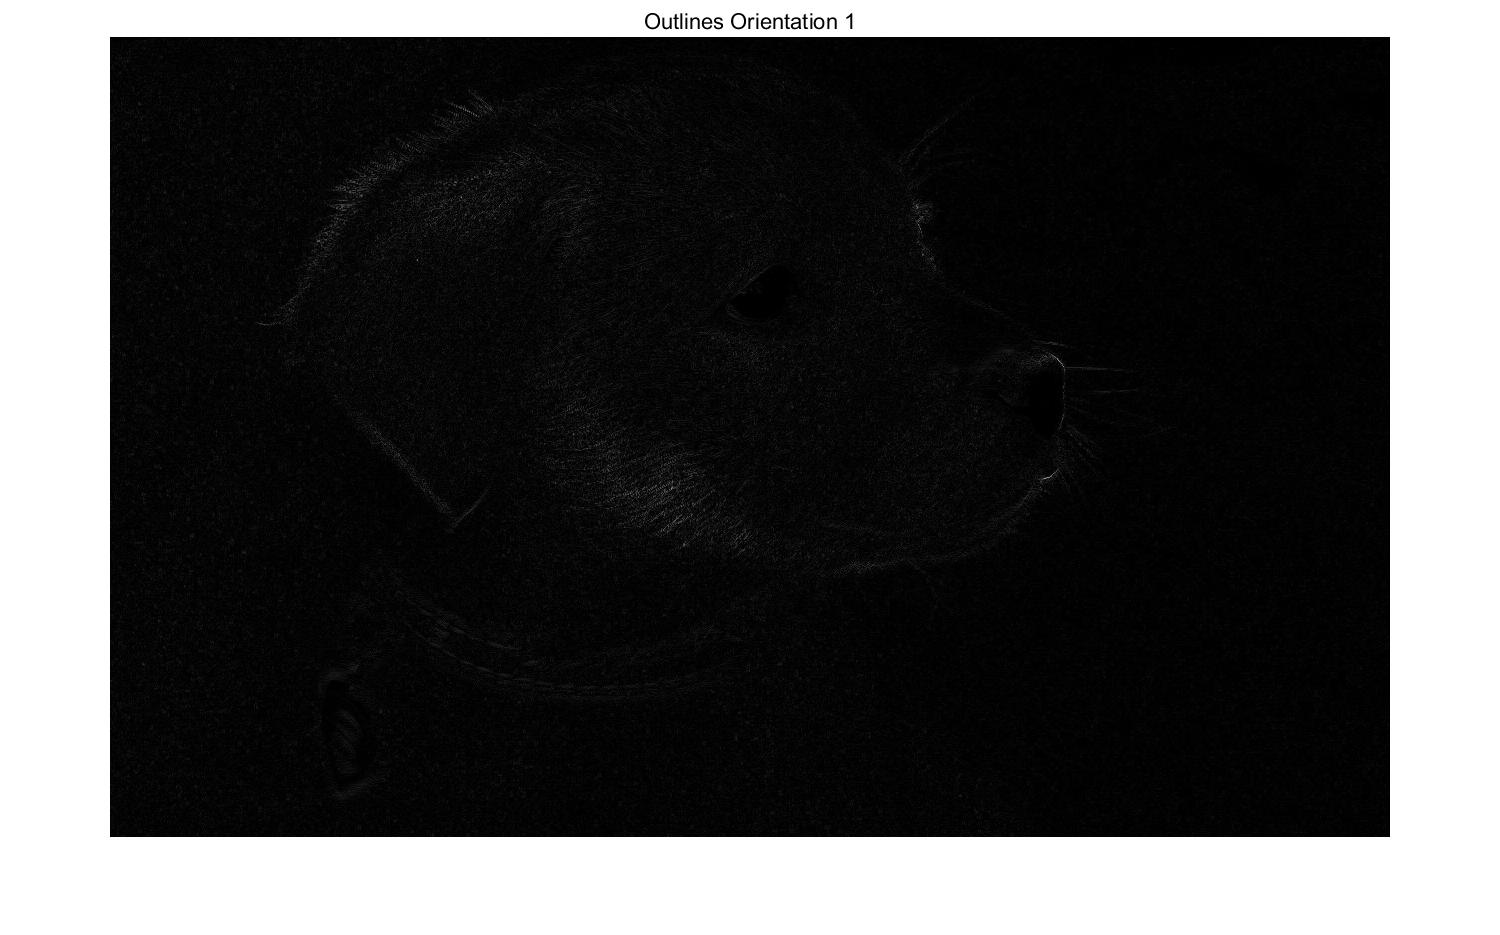
\includegraphics[width=4.0cm]{Ori1.jpg}}
  \centerline{(a) Summation 1}
\end{minipage}
\hfill
\begin{minipage}{0.48\linewidth}
  \centerline{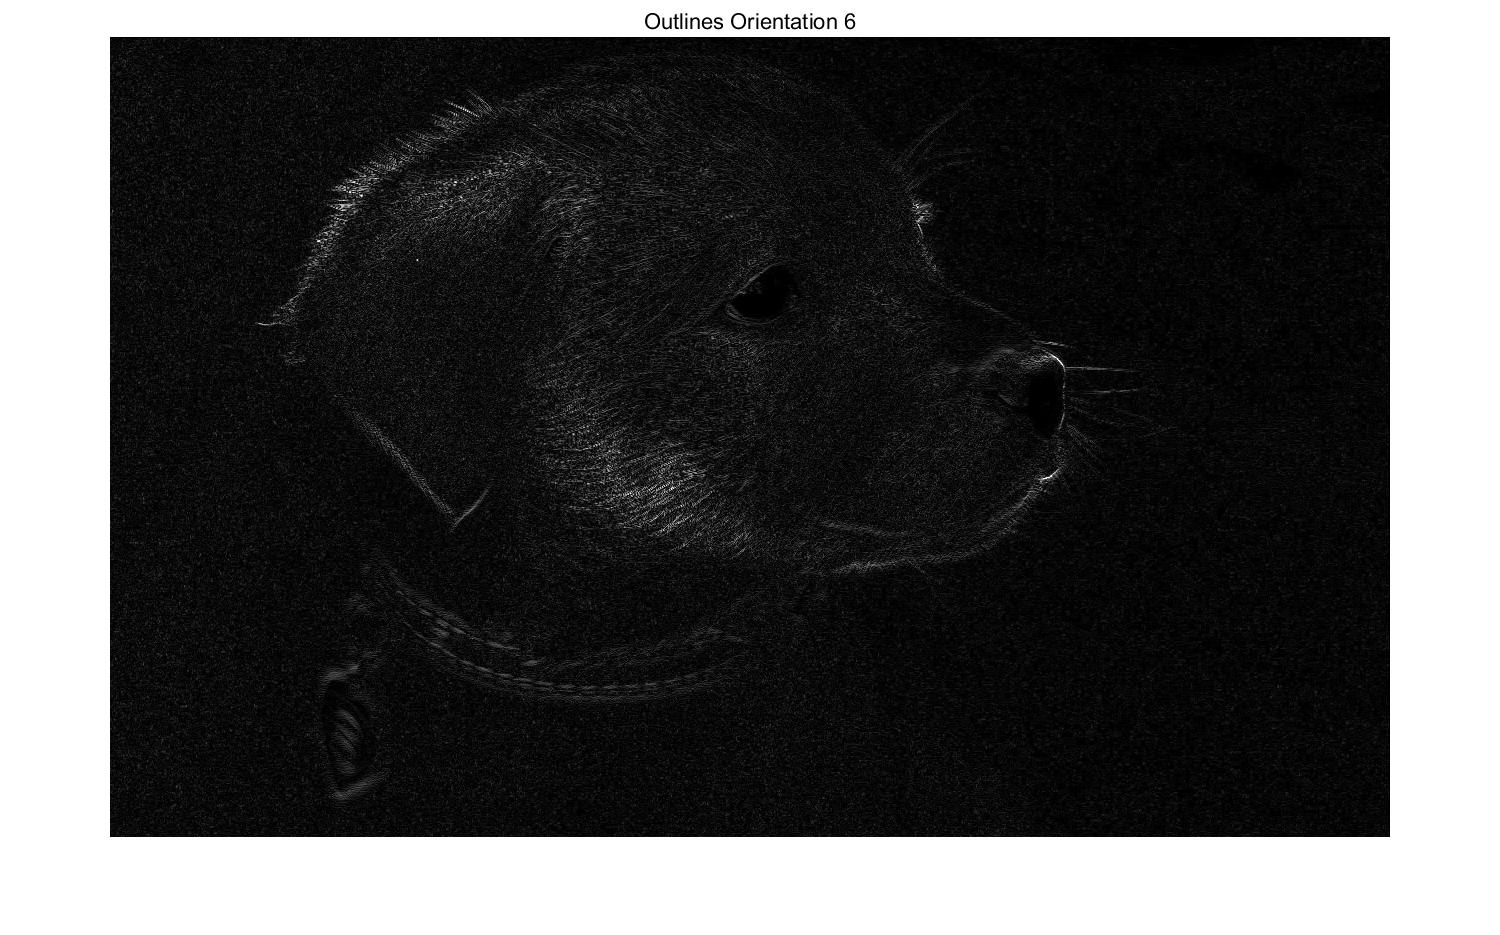
\includegraphics[width=4.0cm]{Ori6.jpg}}
  \centerline{(b) Summation 7}
\end{minipage}
 \caption{Results of Orientation 1 and 7}
\end{figure}

\subsubsection{Adaptive Scheduling}
If the scheduling is composed of n tasks, one of the best scheduling is to maximize the total performance
\begin{equation*}
Q = Q_1(t_1)Q_2(t_2)\cdots Q_n(T-t_1-\cdots-t_{n-1})
\end{equation*}

On the condition that $T = t_1+t_2+\cdots+t_n$. And the optimal solution is obtained by following equations.
\begin{equation*}
\frac{\partial Q}{\partial t_i} = 0 \quad(i=1,2,\cdots,n)
\end{equation*}
% This Performance Profiles are also regarded as Conditional Performance Profiles. And a Conditional Performance Profile denotes the probability of getting a solution of quality when the algorithm is activated with input of quality and execution time.



\section{Workings \&
Discussions of the
Algorithms}
\subsection{Part One}
\subsubsection{Branch \& Bound Algorithm for Solving DLS Problem}

Branch and bound algorithm is one of the trees and graphs traversal and exploring methods. Branch and bound algorithm is performed like blow:
\begin{enumerate}
\item Tree Travers
\item Heuristic function
\item Pruning branches
\end{enumerate}

The algorithm can be described as below: 
  Firstly, all the slaves nodes are put in the first layer. The using the four constraint functions below to minimize T:
\begin{eqnarray}
\sum^{\sigma_a(k)}_{j=1} \alpha_{\sigma_a[j]} +\alpha_kE_k+\sum^m_{j=\sigma_c[j]}C_{\sigma_c[j]}\le \nonumber\\ T (k=1,⋯,m)\\
\sum_{j=1}^m \alpha_{\sigma_a [j]} C_{\sigma_a [j]}+\sum_{j=1}^m\delta \alpha_{\sigma_c [j]} C_{\sigma_c [j]} \le T\\
\sum_{j=1}^m \alpha_j =1\\
 T\ge 0,\alpha_k\ge 0 (k=1,⋯,m) 
\end{eqnarray}

In the above formulation, for the $\sigma_a$, $\sigma_c$ and $\alpha$, the constraint (1) indicates the total time spent in transmission of tasks to all the processors that must receive load before the processor $P_i$ can begin processing its allocated task, the computation time on the processor $P_i$ itself, and the time for transmission back to the source of results of processor $P_i$, and all its subsequent result transfers. For the no-overlap model to be satisfied, the processing time T should be greater than or equal to this time for all them processors. The single-port communication model is enforced by (2) since its LHS represents the lower bound on the time for distribution and collection under this model. The fact that the entire load is distributed amongst the processors is ensured by (3). This is known as the normalization equation. The non-negativity of the decision variables is ensured by constraint (4).
Computing the four constraint functions gets the optimal $\alpha$ and the current processing time by heuristic algorithm. According to the respective processing time, the node with minimum time is selected and other nodes are pruned. Then processing next layer by the same way until all the partitions are arranged, we display this procedure in Figure below.
\begin{figure}[H]
\centering
  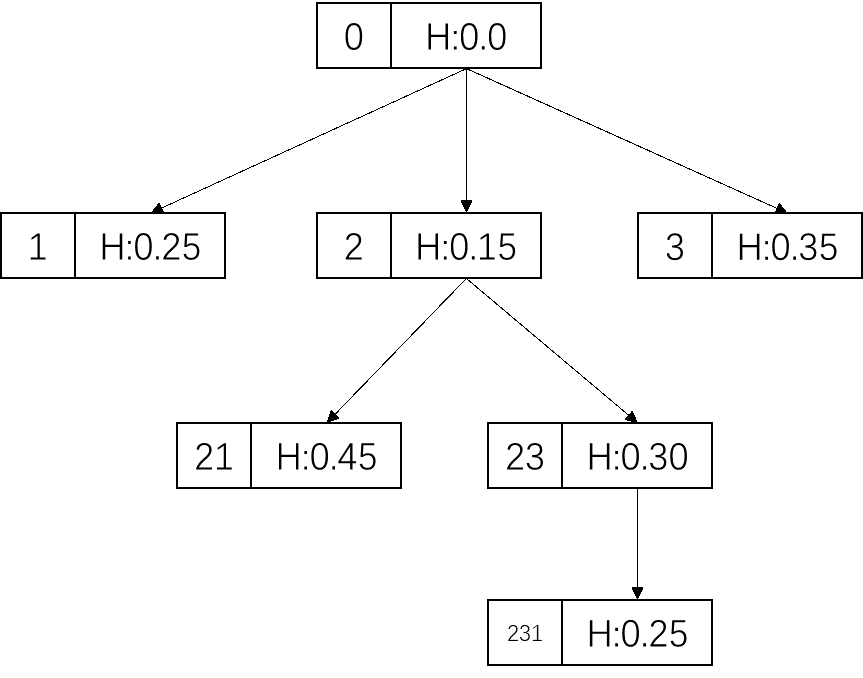
\includegraphics[width=0.4\textwidth]{csn2.png}
\caption{Extending node in Branch and bound}
\end{figure}

In this algorithm (Branch and bound LifoC), the selected computer and its father be located in allocations list hen total slaves that are not appeared in the allocations list, are sorted by increasing C (band width). The collection sequence is list by the inverted order of allocation sequence (list input and first output).

\subsubsection{Comparing with other DLS algorithms}
In this section, I set a group of parameters and compute the result under several DLS algorithms besides Branch and bound LifoC, including ITERLP and FIFOC. The result is showed in Table below.

\begin{table}[h!]
\centering
\begin{tabular}{ ccccc } 
 \hline
 Algorithm & $\sigma_a$ & $\sigma_c$ & $\alpha$ & T\\ 
  \hline
LIFOC&	\{1,2,3\}&	\{3,2,1\}&	\{0.71,0.22,0.07\}&	17.67 \\
ITERLP&	\{1,2,3\}&	\{3,1,2\}&	\{0.61,0.37,0.02\}&	18.04\\ 
FIFOC&\{1,2,3\}&	\{1,2,3\}&	\{0.61,0.36,0.03\}&	18.18\\ 
 \hline
\end{tabular}
\caption{Result for C = {10,15,20}, E = {10,10,1},$\delta$=0.5}
\end{table}
From Table above, we can see that at least in this example the Branch and bound LifoC algorithm is the best.







\subsection{Second Part}
\subsubsection{Algorithm Review}
By modifying processes $P_1,P_2$ and $P_3$ to $P_1',P_2'$ and $P_3'$, respectively, the total time $t_1'+t_2'+t_3'$ becomes less than or equal to T\cite{Anytime}\relax.


\begin{figure}[H]
\centering
  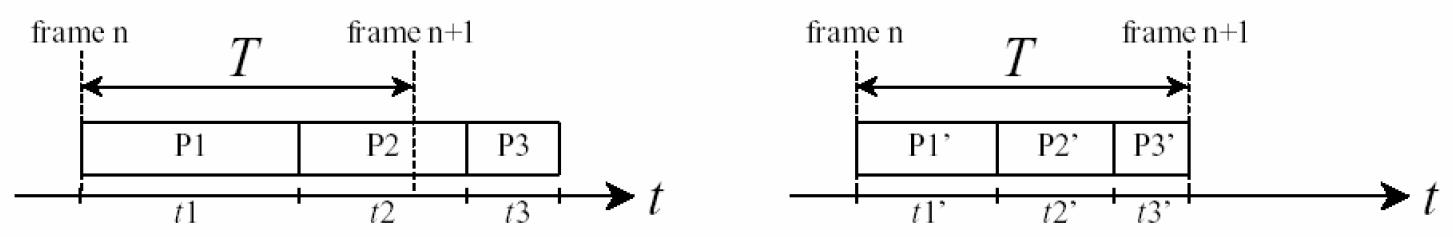
\includegraphics[width=0.4\textwidth]{rel.jpg}
\caption{The Relation Between Restricted Time and Necessary Time for Eacb Process During 1 Frame}
\end{figure}

Image processing is special. Because it can shrink its task load by getting poor performance and it has its special task's sequence which can not arbitrarily change order. Each task has its purpose to get the final results.

\begin{enumerate}[Step 1:]
\item Establish the performance profile function Q(t) to different tasks
\item Decide the sequence of your tasks $Q_1,Q_2,\cdots,Q_n$.
\item Using the time constraint $T = t_1+ t_2 +\cdots+t_n$ to solve the adaptive scheduling function
\begin{equation*}
\frac{\partial Q}{\partial t_i} = 0 \quad(i=1,2,\cdots,n)
\end{equation*}
\item Use $t_i$, get the $max(WCET_i) < t_i$ for each task
\item Implement each task with the operation algorithm corresponding to $t_i$
\end{enumerate}

\subsubsection{Non-trivial Decisions}
Performance Profile functions are typically monotone functions of time, and they can be derived by various curve-fitting techniques. For example $Q(t)=1-e^{-\lambda t}$ to model the expected performance of their anytime planner. It can also be approximated by using a certain family of distributions, even a discrete probability distribution. Here, for calculating simplicity, I use a first order linear function to approximate Performance Profiles.

\subsubsection{Strengths and Pitfalls}
The quality of result is an increasing function. In some cases, we also can use Lagrangian function to solve the optimizing problem with constrains. In my opinion, it may cause the resulting optimal time may get out of the time range, like a negative or a much bigger number. Because now it's a numerical problem. Under those circumstances, when the resulting time is negative, we can choose the least running time. And while the resulting time is a much bigger number, we can run this task with best performance.

In reality, the images may get larger and then get downsized by some certain purposes. For different size image, we should change the WECT. For example, for a larger image, we should multiply a certain parameter to the WECT. It makes sense that processing larger images need more time. So, we should code a program to estimate the image processing task before carrying out it.



\subsection{Comparison Between Our algorithms}
In the second algorithm, it uses multiprocessors with additional communication time, while my partner’s algorithm only uses uniprocessor but allows to reduce the amount of task. So, there exists a critical point where the processing time of two algorithm is same, that is the saving time by minimizing task offsets the advantage of multiprocessors. The parameters which we will discuss are communication time C and $\delta$. Exploring which one is better under different cases.
We limit that the task load is 1 (0.5 task load for each task, total 2 tasks to execute) and the execution time of all the processors used is 10. The number of processors in Branch and bound LifoC algorithm is 3 including one master processor and two slave processors.
First, I fix the communication time of two links is 2 and 5 respectively. The $\alpha$ can be gotten by four constraint equations. Then $\delta$ is the only variable.

\begin{eqnarray}
2\alpha_1+10\alpha_1+2\delta\alpha_1=T \nonumber\\
2\alpha_1+5\alpha_2+10\alpha_2+2\delta\alpha_1+5\delta\alpha_2=T\nonumber\\
\alpha_1+\alpha_2 =1\nonumber
\end{eqnarray}

The relationship between T and $\delta$ is $T=(10\delta^2+90\delta+180)/(25+5\delta)$. The function figure plotting by MATLAB is below. From this figure, we can see that the processing time rises linearly with increasing $\delta$ from 7.2 to 9.33.

\begin{figure}[H]
\centering
  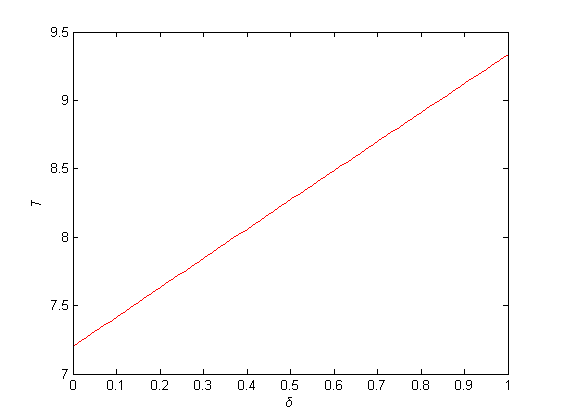
\includegraphics[width=0.4\textwidth]{csn3.png}
\caption{Processing time with $\delta$}
\end{figure}

Second, I fix $\delta=0.5$ and explore the influence on different communication time. The final execution time formula is:
\begin{equation*}
T=(1.5C_1+10)(1.5C_2+10)/(1.5C_2+20) (subject \quad to \quad C_1\le C_2)
\end{equation*}

From this formula, we can get the conclusion about communication time, the communication time of less one has a greater influence on the total execution time ( $C_1$ in this assumption). 


While for the second part, I also take two tasks each for 0.5 task load, runtime for each unit amount of task load is 10. After applied the constraint $t_1 + t_2 = T$, via the adaptive scheduling equation, we could get the optimal execution time for each task:
\begin{eqnarray}
t_1 = 0.4994T+0.2246 \nonumber \\
t_2 = 0.5006T-0.2246 \nonumber
\end{eqnarray}

Also, from the table of the algorithm 1, we could know, for two tasks, one for detection edge and one for smoothing, the total execution time should be at least 2.5 and the longest time should be 10 which will lead to best performance.

\begin{figure}[H]
\centering
  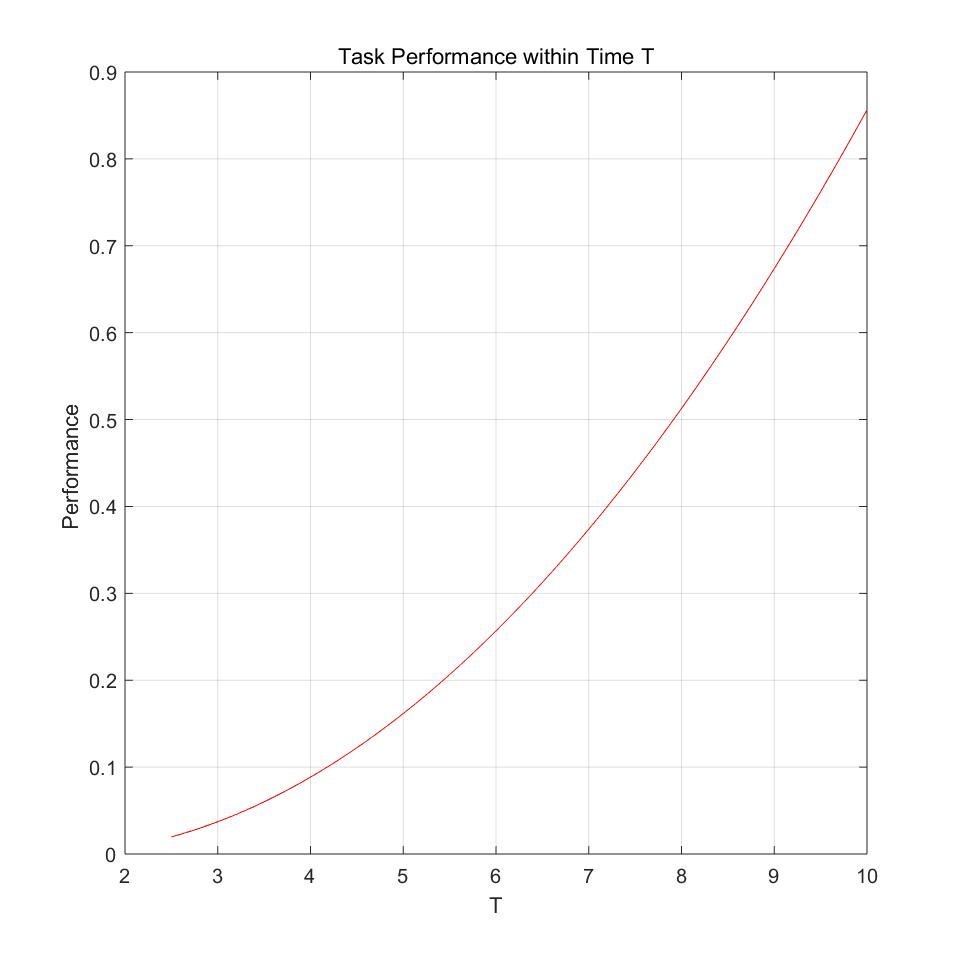
\includegraphics[width=0.4\textwidth]{perf.jpg}
\caption{Image Processing Task Performance}
\end{figure}

Compared to the first algorithm, we could see, both algorithms have applied the special features of image processing, but the second algorithm could implement the algorithm with the execution time 2.5! Instead, the first algorithm need at least 7.2 time to run the program.

\section{Conclusion} 
In this report, we survey two real time algorithms for image processing. Both take advantage of the features of image processing. First one is that image can be segmented into several pieces, and the second one bases on that image processing can be simplifying. Branch and bound LifoC algorithm achieve high performance on heterogeneous network systems. 

If we have plenty of time, the first algorithm is a better choice. Otherwise, the second algorithm can solve the lacking time problem by sacrificing the image processing quality. By comparison, when our time limit is more than 7.5, we should choose the first algorithm, which give us the best performance. Although, the first algorithm gives us the image processing results too, the resulting images has poorer performance. When the time gets strict limit, we prefer the second algorithm instead.

The author successfully solve this kind of problem. Furthermore, it makes us think of Convolution Neuron Network. An algorithm calls Drop-Out. It also ignores some parameters in the mask brick, which aims to regularize the parameters and avoid over-fitting. Now, it seems to save some time too!

Maybe, in future, we will explore the possibility to combine the two algorithms, which may give us a better results under strict time confine.


\begin{thebibliography}{unsrt}
  \bibitem{Using anyt}
    Shlomo Zilberstein \emph{Using Anytime Algorithms in Intelligent Systems} (AI Magazine, Volume 17 Number 3, 1996).
    \bibitem{Anytime}
    Wyne Wyne Kywe \& Daisuke Fujiwara \emph{Scheduling of Image Processing Using Anytime Algorithm for Real-time
System} (The 18th International Conference on Pattern Recognition).
\bibitem{Distributed}
    Farzad N.\&  Farzad M.\emph{Distributed Image Processing Scheduling in Heterogeneous Computing Network System} (2012).
    \bibitem{devisi}
    Ghatpandc A. \& Nakazato H. \emph{Divisiblle Load Scheduling with Result Collection on Heterogeneous Systems} (Proc. Heterogeneous Comuting Workshop, HCP, 2008).

\end{thebibliography}



\end{document}
\section{Abstract}
Using an algorithm called anytime algorithm to greatly enhance the performance of the image processing in the restricted time.

T-p
Real-time image processing for motion planning and distance estimation based on stereo camera images. Ensuring hard real-time with complex algorithms on modern computer architectures is difficult to realize due to unpredictable execution times of algorithms with data dependent runtime. This new scheduling scheme allows to use Anytime algorithm
\section{Introduction}
The quality of image processing is usually evaluated by high extraction rate or low error rate. Although many approaches from processing time are reported in the region of system planning in AI, there are few reports in the scheduling of image processing.

The algorithm intends to perform individual image processing task at optimal time. It is also describes an evaluation method under such a condition that the processing time is restricted or is not enough, and proposes an adaptive scheduling method by using anytime image processing.

Task-pair:

Nearly all classical real-time scheduling approaches rely on the knowledge of the Worst Case Execution Times (WCETs) for all tasks of the system. The Expected Case Execution Time (ECET) is used instead to accomplish a better CPU load. The entire algorithm must be modified in a way to make first results available after a short time and to improve them during further execution time. After the first calculated result is available the task may be interrupted in case of a possible deadline violation, keeping a guaranteed calculation result.

\section{Anytime Algorithm for Real-time Image Processing}
\subsection{Outline of Anytime Algorithm}
In real time image processing system, a good scheduling algorithm should offer a trade-off between computation time and the quality of result returned. 

If each process could return the result anytime, the total processing time would be reduced in restricted time even though the quality is not perfect.

Anytime algorithm is a method that the precision or accuracy of the result will be improved according to the increase of computation time, and this is reported mainly in the field of AI. The accuracy will be improved according to the increase of computation like the Newton's method.

T-p: 

idea of using estimated execution times that are based on statistics and system monitoring instead of fixed WCETs. The 







